\chapter{wells}
\label{sec:wells}
\lhead[tempest]{}
\lstset{style=6502Style}

Wells are fun and should be easy to draw. To start with, we can describe a 2d shape
of our choice using a bunch of x/y co-ordinates as points.
\begin{figure}[H]
    \centering
    \begin{adjustbox}{width=7cm,center}
      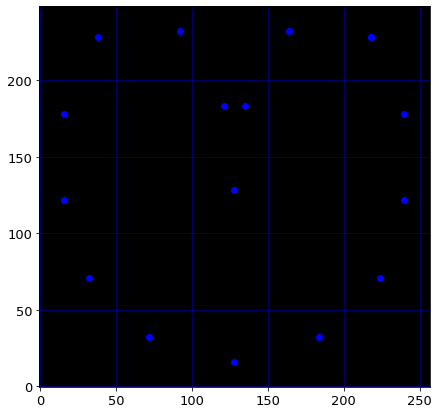
\includegraphics[width=12cm]{src/wells/HEART_dots_no_title.png}%
    \end{adjustbox}
  \caption{Make our dots.}
\end{figure}

Next we can join these together to give us a 2d shape.
\begin{figure}[H]
    \centering
    \begin{adjustbox}{width=8cm,center}
      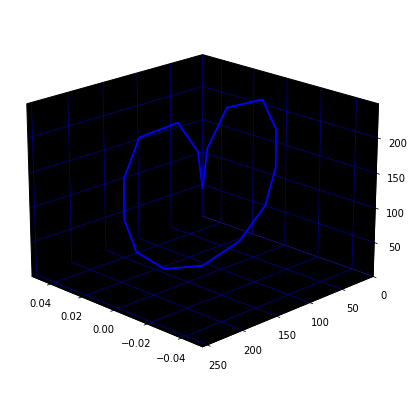
\includegraphics[width=12cm]{src/wells/HEART_2d.png}%
    \end{adjustbox}
  \caption{Start with a 2d shape..}
\end{figure}

To make this thing three dimensional all we have to do is project our shape onto
some chosen distant position along the Z plane.
\vspace{-0.5cm}
\begin{figure}[H]
    \centering
    \begin{adjustbox}{width=8cm,center}
      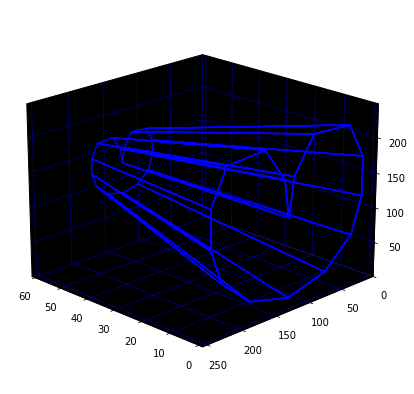
\includegraphics[width=12cm]{src/wells/HEART_3d.png}%
    \end{adjustbox}
  \caption{..then make it three dimensional.}
\end{figure}

Seems simple enough. With this as our objective the data structure below gives us
everything we need to create the web. In addition to listing the 16 vertices that
make up the web's shape in two dimensions.

\begin{lstlisting}
; Data structure for the 'HEART' well. 
; X Co-Ordinates
    .BYTE 0DA,0A4, 87, 80, 79, 5C, 26, 10    ;HEART
    .BYTE  10, 20, 48, 80,0B8,0E0,0F0,0F0
; Y Co-Ordinates
    .BYTE 0E4,0E8,0B7, 80,0B7,0E8,0E4,0B2     ;HEART
    .BYTE  7A, 47, 20, 10, 20, 47, 7A,0B2
\end{lstlisting}

To help you relate this table to the co-ordinates in our graphs let's list
it in decimal instead:
\begin{lstlisting}
; Data structure for the 'HEART' well. 
; X Co-Ordinates
    .BYTE 218,164,135,128,121, 92, 38, 16    ; HEART
    .BYTE  16, 32, 72,128,184,224,240,240
; Y Co-Ordinates
    .BYTE 228,232,183,128,183,232,228,178    ; HEART
    .BYTE 122, 71, 32, 16, 32, 71,122,178
\end{lstlisting}

\begin{lstlisting}
        .SBTTL  UTILITY-DRAW WELL SHAPE
DSPHOL:
        JSR LVLWEL              ;SET UP WELL INDEX & ID
        STA SAVEY               ;WELL INDEX
        STX SAVEX               ;CYCLE
        LDA I,0
        STA VGBRIT
        LDA I,5                 ;MAKE WELL REALLY SMALL
        JSR VGSCA1
        LDA SAVEX               ;GET CYCLE (TIMES THRU ALL WELLS
        AND I,7
        TAX
        LDY X,SPWECO            ;GET SPECIAL WELL COLOR FOR CYCLE
        STY COLOR
        LDA I,MZCOLO
        JSR VGSTAT              ;SET WELL COLOR
        LDX WELLID
        LDA SAVEY
        LDY X,HOLRAP
        IFEQ                    ;PLANAR?
        SEC                     ;NO. START BEAM AT FIRST POINT
        SBC I,0F                ;IN TABLE (FOR CLOSED WELLS)
        ENDIF
        TAY
        LDA Y,NEWLIZ
        STA PYL
        EOR I,80                ;ADJUST Z SIGN
        TAX
        LDA Y,NEWLIX            ;SAVE COORDS OF 1ST PT
        STA PXL
        EOR I,80                ;ADJUST X SIGN
        JSR VGVTR1              ;POSITION BEAM AT 1ST PT ON WELL
        LDA I,0C0               ;TURN BEAM ON
        STA VGBRIT
        LDX I,NLINES-1
        STX INDEX2
        BEGIN                   ;LOOP FOR EACH PT ON EDGE
        LDY SAVEY
        LDA Y,NEWLIX            ;
        TAX
        SEC
        SBC PXL                 ;DELTA X
        PHA                     ;
        STX PXL                 ;CURRENT X OLD X
        LDA Y,NEWLIZ
        TAY
        SEC
        SBC PYL                 ;DELTA Z
        TAX
        STY PYL                 ;CURRENT Z>OLD Z
        PLA
        JSR VGVTR1              ;DRAW VECTOR TO NEXT PT.
        DEC SAVEY
        DEC INDEX2
        MIEND
        LDA I,1                 ;NORMAL SIZE AGAIN
        JMP VGSCA1
\end{lstlisting}
